\documentclass[11  pt]{article} 
\usepackage[lmargin=1in,rmargin=1.75in,bmargin=1in,tmargin=1in]{geometry}  


% For hyperlinking everything
\usepackage{hyperref}
\hypersetup{
	colorlinks=true, %set true if you want colored links
	linktoc=all,     %set to all if you want both sections and subsections linked
	linkcolor=blue,  %choose some color if you want links to stand out
}


\usepackage[latin1]{inputenc}
\usepackage{amsmath}
\usepackage{mathrsfs}  
\usepackage{amsfonts}
\usepackage{amssymb}
\usepackage{graphicx}
\usepackage{subfig}
\usepackage{caption}
\usepackage{algorithm}
%\usepackage{algcompatible}
%\usepackage{algorithmicx}
\usepackage{algpseudocode}

\usepackage{titlesec}
\titleformat{\section}{\fontfamily{lmss}\fontsize{14}{15}\bfseries}{\thesection}{1em}{}
\titleformat{\subsection}{\fontfamily{lmss}\fontsize{12}{15}\bfseries}{\thesubsection}{1em}{}




\usepackage{amsthm}

\newtheoremstyle{noit}
{10pt}% <Space above>
{10pt}% <Space below>
{}% <Body font>
{}% <Indent amount>
{\bfseries}% <Theorem head font>
{.}% <Punctuation after theorem head>
{.5em}% <Space after theorem headi>
{}% <Theorem head spec (can be left empty, meaning `normal')>

\newtheoremstyle{example}
{10pt}% <Space above>
{10pt}% <Space below>
{}% <Body font>
{20pt}% <Indent amount>
{\bfseries}% <Theorem head font>
{.}% <Punctuation after theorem head>
{.5em}% <Space after theorem headi>
{}% <Theorem head spec (can be left empty, meaning `normal')>


\newtheoremstyle{indented}{20pt}{20pt}{\addtolength{\leftskip}{2.5em}}{}{\bfseries}{.}{.5em}{}


\newtheorem{theorem}{Theorem}
\numberwithin{theorem}{section}
\newtheorem{lemma}[theorem]{Lemma}
\newtheorem{corollary}[theorem]{Corollary}
\newtheorem{observation}{Observation}
%\numberwithin{observation}{section}
%\numberwithin{definition}{section}
\newtheorem{conjecture}{Conjecture}
\newtheorem{Qu}{Question}
\newcommand{\QU}{\begin{Qu}\normalfont}

\theoremstyle{noit}
\newtheorem{fact}{Fact}
\newtheorem{definition}{Definition}

\theoremstyle{indented}
\newtheorem{example}{Example}

\theoremstyle{indented}
\newtheorem{problem}{Problem}


%\newenvironment{proof}{\noindent{\bf Proof:} \hspace*{1em}}{
%    \hspace*{\fill} $\Box$ }
%\newenvironment{proof_of}[1]{\noindent {\bf Proof of #1:}
%    \hspace*{1em} }{\hspace*{\fill} $\Box$ }
%\newenvironment{proof_claim}{\begin{quotation} \noindent}{
%    \hspace*{\fill} $\diamond$ \end{quotation}}
\newcommand{\vs}[1]{\vspace{#1}}

\newcommand{\lecture}[2]{
 \noindent
\begin{center}
	\framebox{
		\vbox{
			\hbox to 5.78in { {\bf CSCE 411: Design and Analysis of Algorithms} \hfill  }
			\vspace{2mm}
			\hbox to 5.78in { {\Large \hfill Lecture #1\hfill} }
			\vspace{2mm}
			\hbox to 5.78in { {\it Date: #2 \hfill Lecturer: Nate Veldt} }
		}
	}
\end{center}
\vspace*{4mm}
}


\newcommand{\hw}[2]{
	\noindent
	\begin{center}
		\framebox{
			\vbox{
				\hbox to 5.78in { {\bf CSCE 411: Design and Analysis of Algorithms} \hfill  }
				\vspace{2mm}
				\hbox to 5.78in { {\Large \hfill Homework #1\hfill} }
				\vspace{2mm}
				\hbox to 5.78in { {\it Due date: #2 \hfil} }
			}
		}
	\end{center}
	\vspace*{4mm}
}



\newcommand{\under}[1]{\underline{\hspace{#1}}}
\setlength{\parindent}{0em}

%\usepackage[tagged]{accessibility}

% Graph terms
\newcommand{\vol}{\textbf{vol}}
\newcommand{\cut}{\textbf{cut}}


% Matrices
\newcommand{\mA}{\textbf{A}}
\newcommand{\mB}{\textbf{B}}

% vectors
\newcommand{\ve}{\textbf{e}}
\newcommand{\vx}{\textbf{x}}


% Other
\newcommand{\calN}{\mathcal{N}}

\usepackage{mathtools}
\DeclarePairedDelimiter\ceil{\lceil}{\rceil}
\DeclarePairedDelimiter\floor{\lfloor}{\rfloor}


\newcommand*{\aitem}{ \item[{
\includegraphics[width=0.8cm,height=0.5cm]{../../Lectures/figures/A}} ]  }
\newcommand*{\bitem}{ \item[{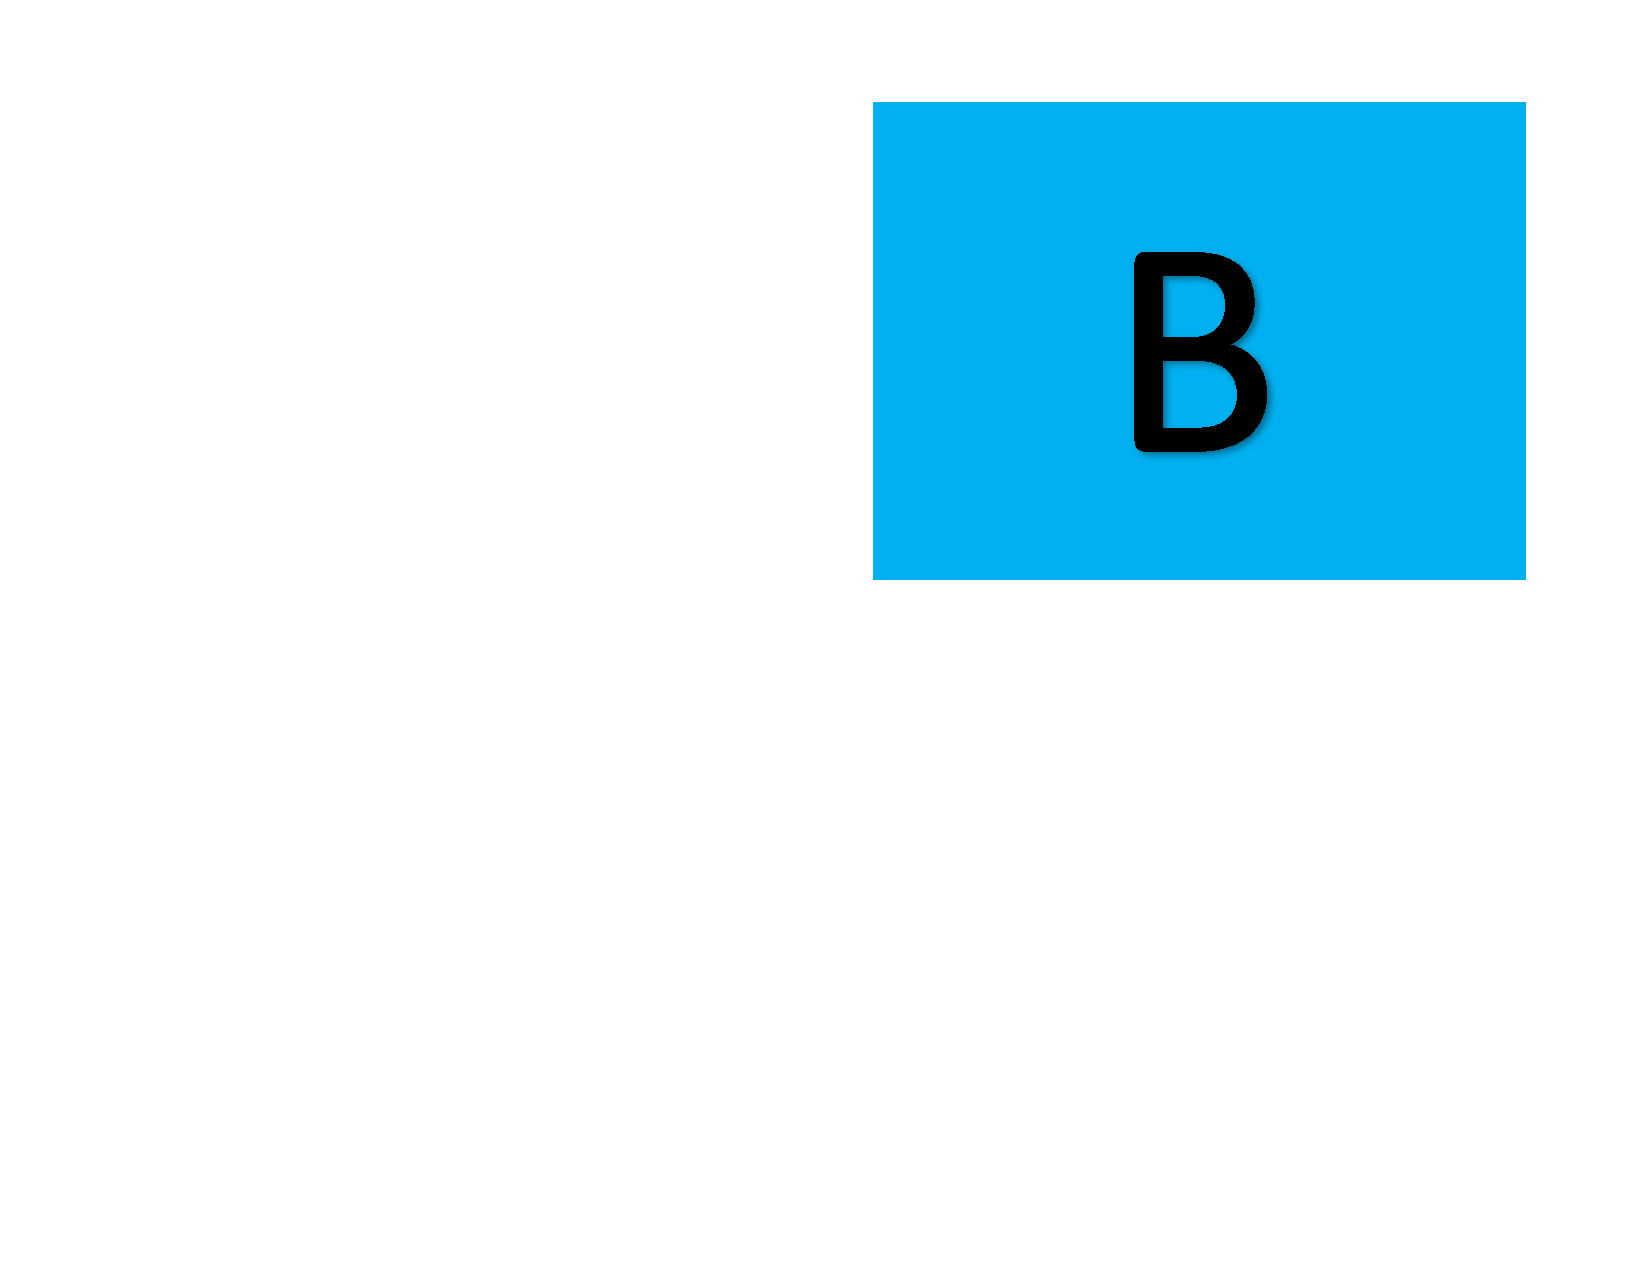
\includegraphics[width=0.8cm,height=0.5cm]{../../Lectures/figures/B}} ]  }
\newcommand*{\citem}{ \item[{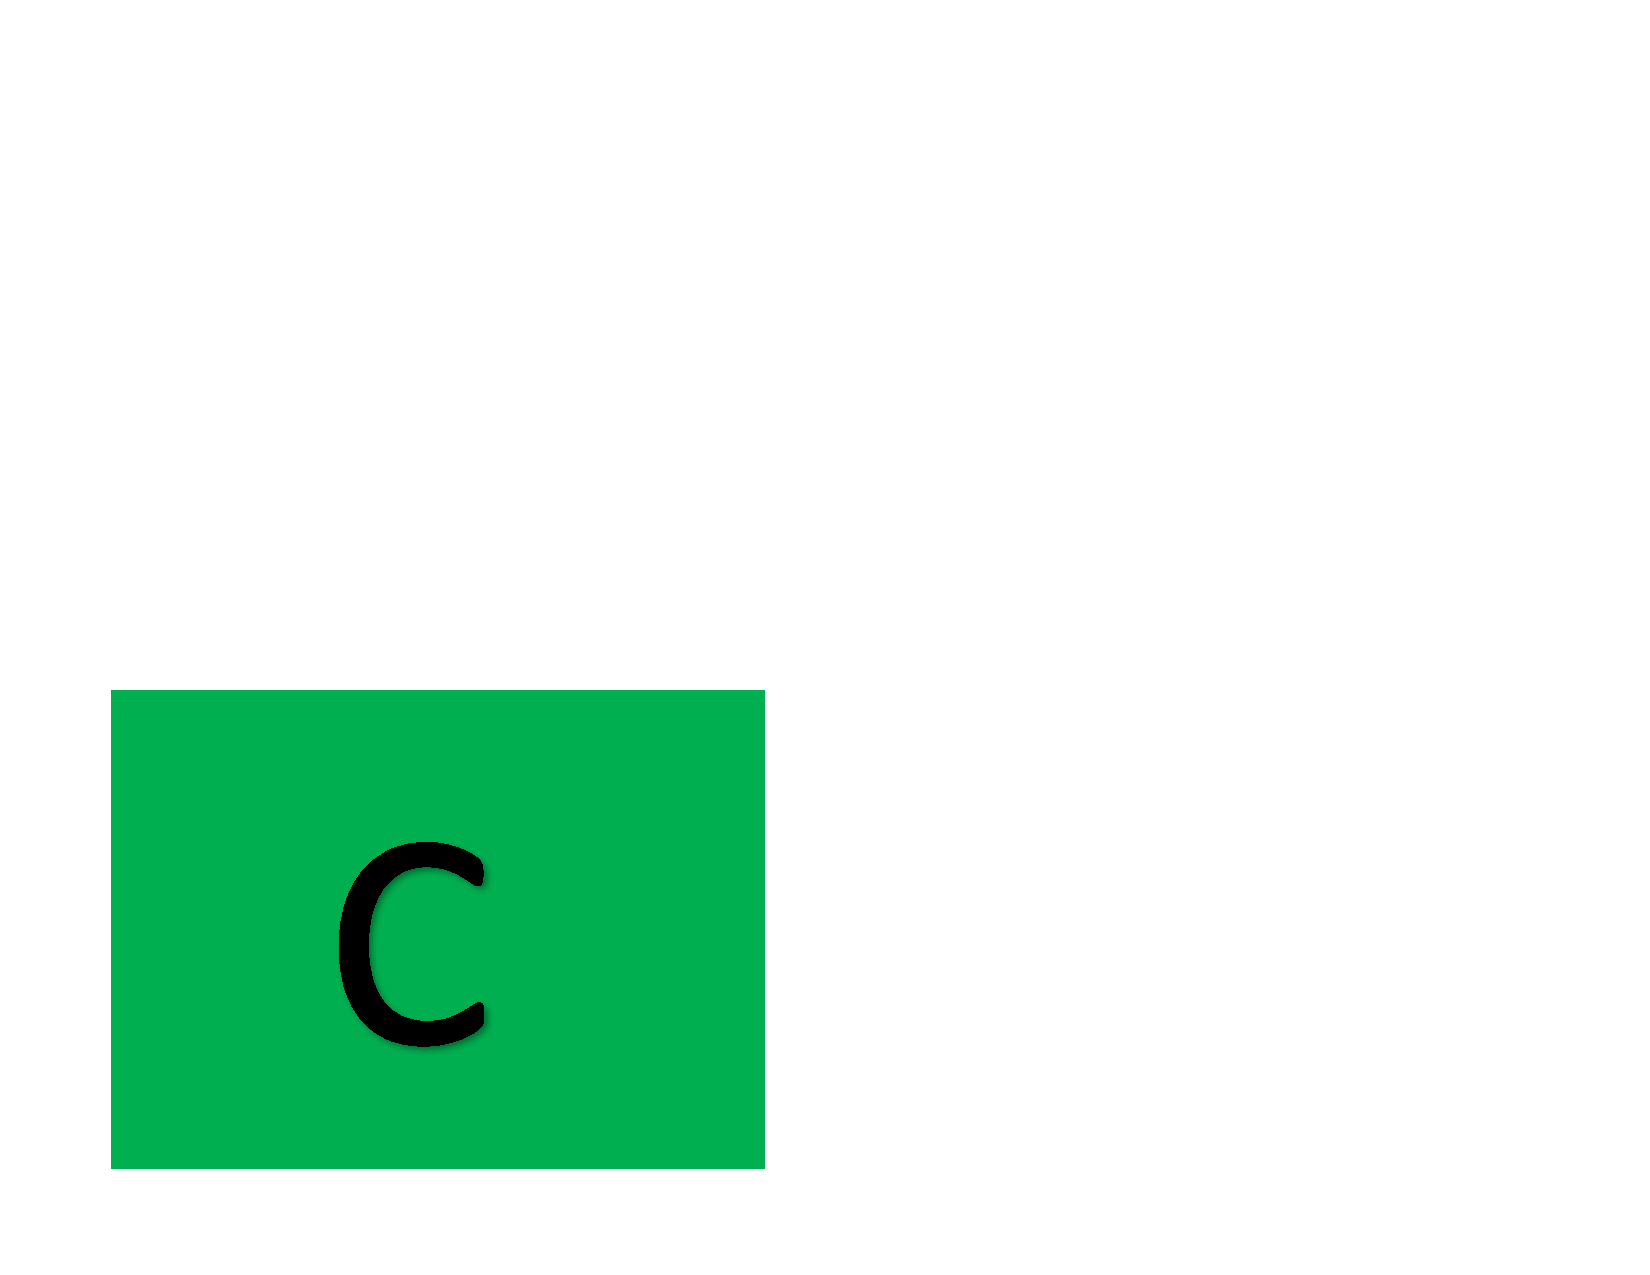
\includegraphics[width=0.8cm,height=0.5cm]{../../Lectures/figures/C}} ]  }
\newcommand*{\ditem}{ \item[{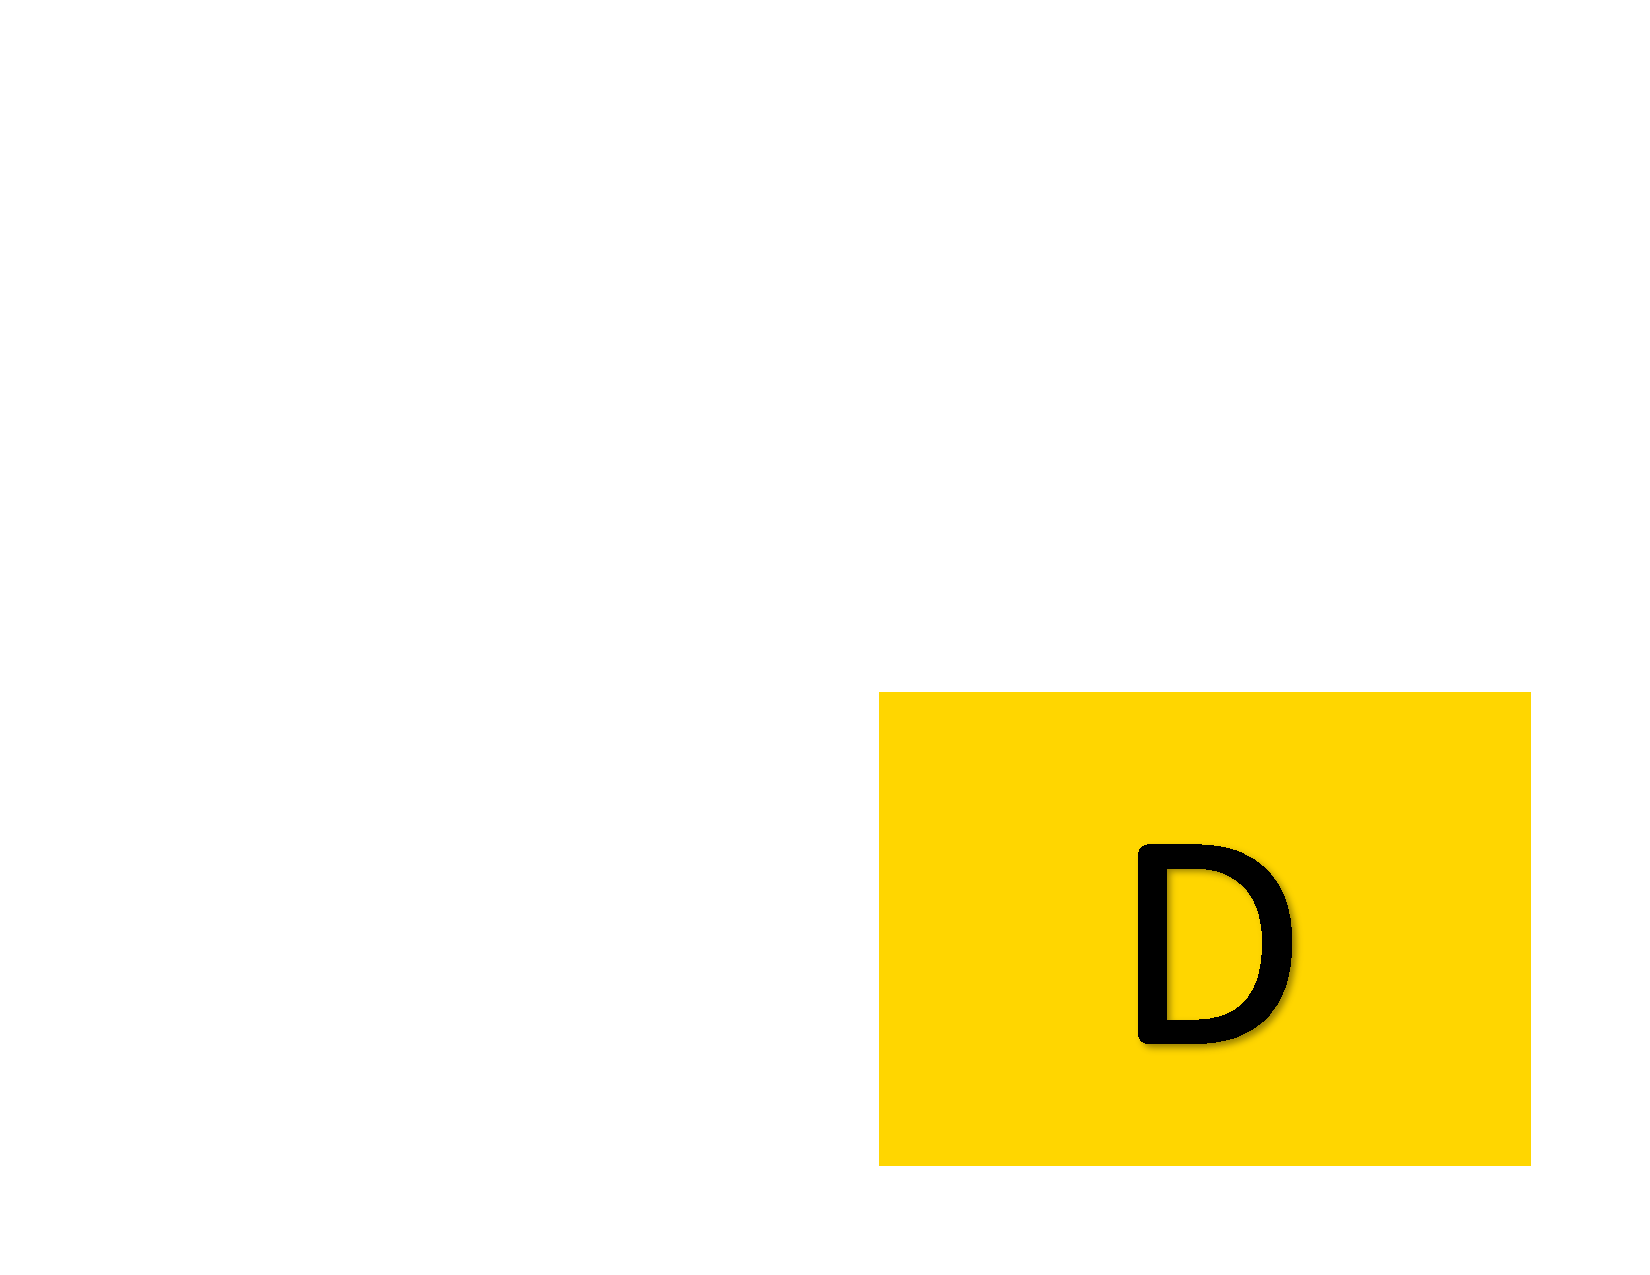
\includegraphics[width=0.8cm,height=0.5cm]{../../Lectures/figures/D}} ]  }
\newcommand*{\eitem}{ \item[{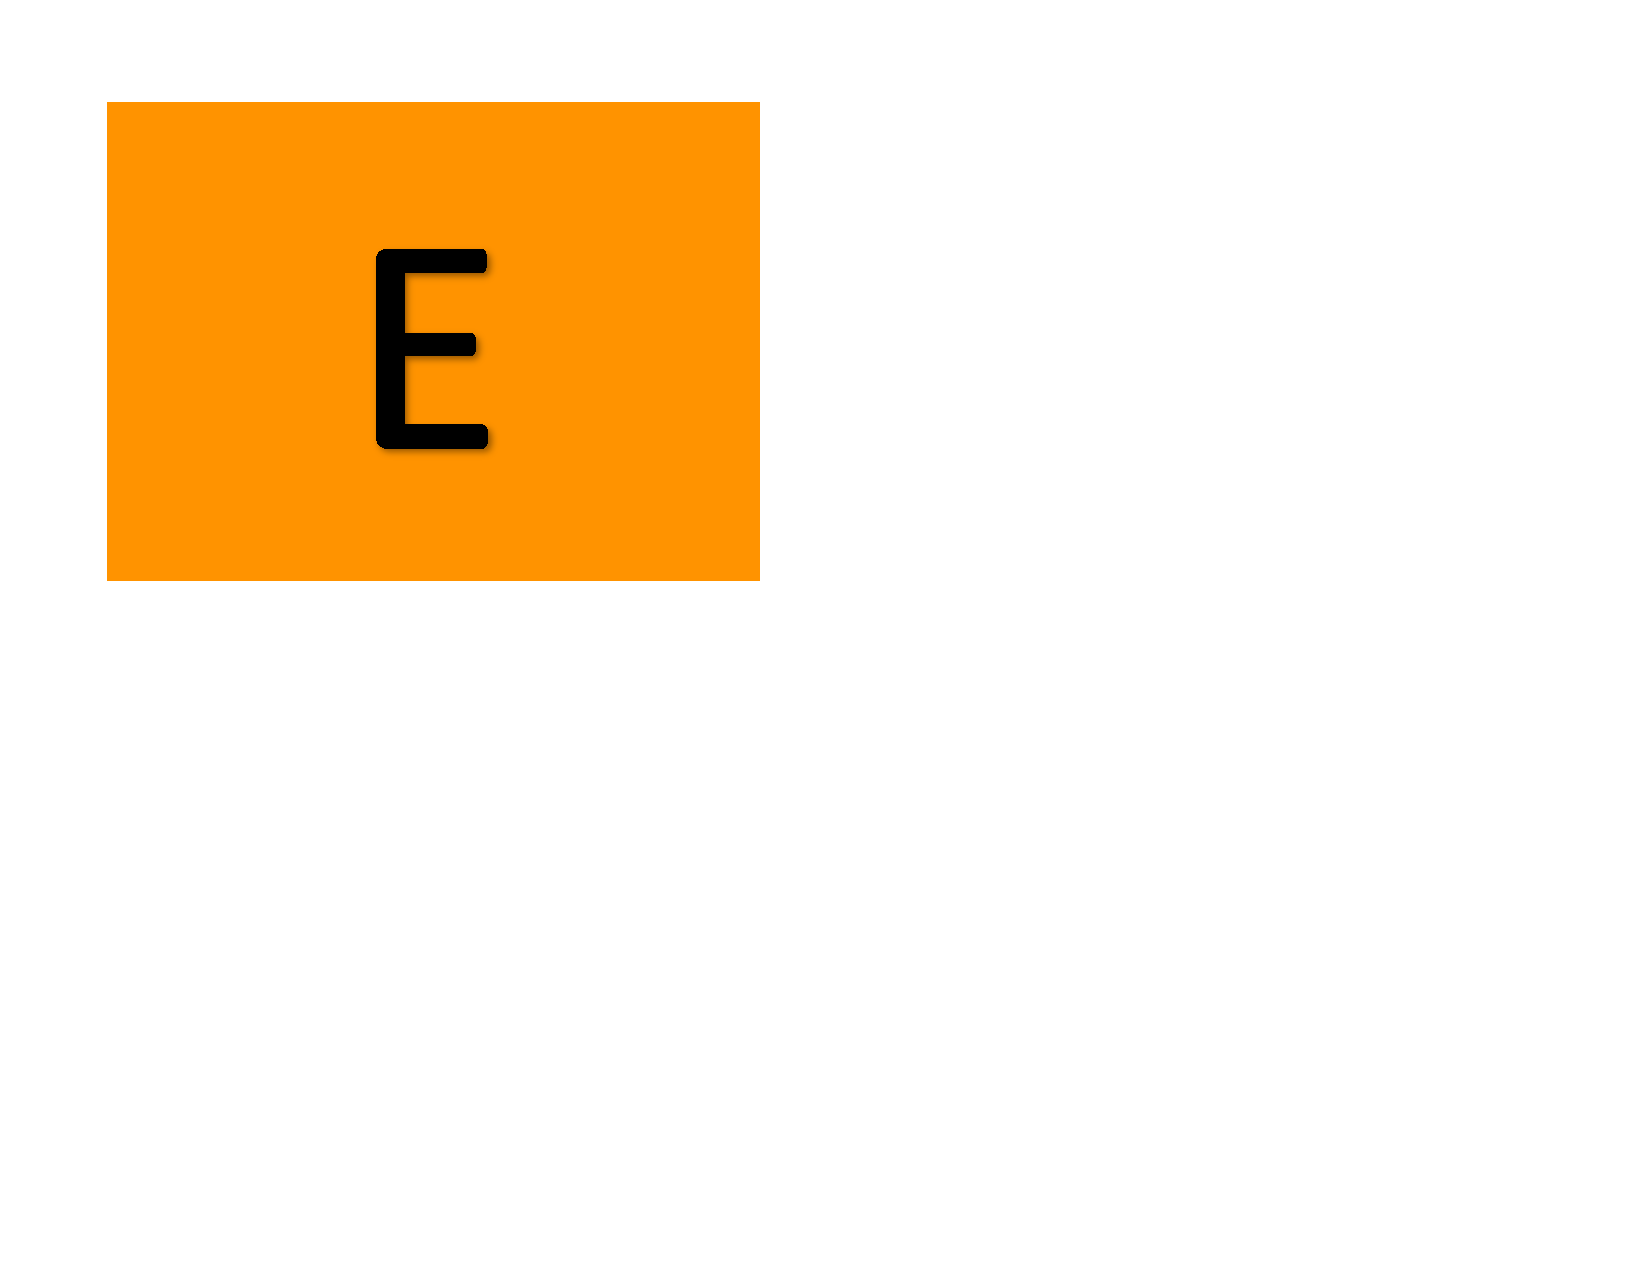
\includegraphics[width=0.8cm,height=0.5cm]{../../Lectures/figures/E}} ]  }
\newcommand*{\fitem}{ \item[{
\includegraphics[width=0.8cm,height=0.5cm]{../../Lectures/figures/F}} ]  }


\newcommand{\hide}[1]{\underline{\phantom{#1 #1}}}

\usepackage{setspace}

\onehalfspacing

\begin{document}
	
	\lecture{22: co-NP, Reductions, NP-completeness}{Week 13}
	
	\section{The co-NP class}
	A problem is in co-NP if for every \hide{NO instance } there is a \emph{certificate} (some data) that an algorithm can use to \emph{verify} in polynomial time that it is truly a \hide{ NO instance.} \\ \\
	
	To be clear, we will often use the terms \hide{NO}-certificate and \hide{NO}-verifier. \\ \\
	
	
	\textbf{Example problem} Is $G = (V,E)$ a directed acyclic graph? \\ \\
	
	\vs{2cm}
	
	\textbf{Certificate} \\ \\ %A set of nodes that defines a cycle. \\ \\
	
	\vs{2cm}
	
	\textbf{Verifier} \\ \\ %Check that the set of nodes is a cycle. \\ \\
	
	
	\vfill
	
	\textbf{Conclusion}: Checking whether $G$ is a DAG is \hide{in co-NP. }  \\
	\vs{1cm}
	
	\newpage
	
	\begin{Qu}
		The verifier we showed for the clique problem will return YES if the $k$ nodes are a clique, and will return NO if the $k$ nodes are not a clique. \\
		
		True or false: this means that this algorithm is also a NO-verifier, and so the clique problem is also in co-NP.
		\begin{itemize}
			\aitem True
			\bitem False
		\end{itemize}
		
		
	\end{Qu}
	
	\vfill
	
	\begin{Qu}
		Checking whether $G$ is a DAG in in co-NP. Is it also in NP? 
		\begin{itemize}
			\aitem Yes
			\bitem No
		\end{itemize}
		
	\end{Qu}
	\vfill
	\newpage
	\section{Reductions}
	A reduction is a mapping from one computational problem to another.  \\ 
	
	\textbf{Definition} Let $A$ and $B$ be decision problems. We say that $A$ can be reduced to $B$ if
	
	\begin{itemize}
		\item For every instance of $A$ we can define a corresponding instance of $B$ such that
		\item All YES instances in $A$ map to YES instances in $B$
		\item All NO instances in $A$ map to NO instances in $B$
	\end{itemize}
	
	\vfill
	
	This is a polynomial-time reduction if this conversion process takes polynomial time. \\
	
	This seems obvious: what's an example of a reduction that is not polynomial-time? \\ \\
	
	\vfill
	
	\newpage
	\subsection{Reduction and complexity}
	
	If $A$ can be reduced to $B$ in polynomial time, we denote this by 
	
	\begin{equation*}
		\hide{A \leq_p B}
	\end{equation*}
	
	This implies that:
	\begin{itemize}
		\item $A$ is easier\footnote{where easier might mean ``no harder than''} than $B$, or equivalently 
		\item $B$ is at least as hard as $A$ is to solve\\
	\end{itemize} 
	
	\begin{lemma} 
		If $B \in P$ and \hide{$A \leq_p B$}, then \hide{ $A \in P$.}
	\end{lemma}	
	
	\newpage
	
	
	\section{NP-completeness}
	
	\textbf{Definition: } A problem $Q$ is NP-complete if:
	\begin{enumerate}
		\item $Q \in$ NP
		\item for every problem $B \in \text{NP}$, $B \leq_p Q$. \\
	\end{enumerate}
	
	\textbf{In words:} \\ %a problem is NP-complete if it is NP and you can reduce any problem in NP to it. \\
	
	
	\vs{8cm}
	
	This implies that NP-complete problems are the \emph{hardest} problems in NP. \\
	
	
	Why? Remember that $A \leq_p B$ means $A$ is easier than $B$. \\
	
	In fact, if you only take the second part of the definition, this defines the set of NP-hard problems.
	
	
	\newpage
	
	\section{Views of the computational problem universe}
	There are four different possibilities for the relationship between P, NP, and co-NP.
	
	
	
	\vfill
	
	There are two possibilities for the relationship between P, NP, and NP-complete.
	
	\vfill
	
	\newpage
	
	\paragraph{A few famous NP-complete problems}
	\begin{itemize}
		\item Find if a graph has a clique of size at least $k$
		\item Find if a graph has a Hamiltonian cycle
		\item Find if a graph has a simple path with at least $k$ edges
		\item \textbf{Subset sum}: given a set of numbers, find if any subset sums to zero
		\item \textbf{SAT}: Logic problems we will look at in more depth later
	\end{itemize}
	
	
	\section{Summary on Reduction and NP-completeness}
	If $A$ can be reduced in polynomial time to $B$, we write $A \leq_p B$. This means that $A$ is no harder than B; a solver for $B$ can be used to solve $A$.\\
	
	\vs{2cm}
	\vfill
	
	A problem $Q$ is NP-hard if every problem in NP can be reduced to $Q$ in polynomial time. \\
	
	A problem $Q$ is NP-complete if
	\begin{itemize}
		\item It is in NP
		\item It is NP-hard\\
	\end{itemize}
	
	\vfill
	
	
	\begin{Qu}
		Assume that $A$ and $B$ are both in NP and $A \leq_p B$. Which of the following statements is false?
		\begin{itemize}
			\aitem If $A \in \text{P}$, then $B \in \text{P}$
			\bitem If $A$ is NP-complete, then $B$ is NP-complete
			\citem If $B \in \text{P}$, then $A \in \text{P}$
			\ditem If $A$ is NP-complete, then $B \leq_p A$
		\end{itemize}
	\end{Qu}
	\vs{1cm}
	
	If two problems are NP-complete, then they are both in NP, and:
	
	\vs{1cm}
	
	\newpage
	
	\section{Why does it matter whether a problem is in P, NP, or is NP-complete?}
	%There are lots of problems we want to know how to solve with a computer. When we encounter a new problem, it's helpful to know how inherently challenging the problem is! \\
	
	A famous book by Garey and Johnson, \emph{Computers and Intractability}, includes some famous cartoons to help us answer this question.\footnote{Garey, Michael R., and David S. Johnson. Computers and intractability. Vol. 174. San Francisco: freeman, 1979. High-resolution versions of the cartoon are available online. }\\
	
	Let's say your boss tells you that because you are a CS major or minor you should be able to find an efficient algorithm for a certain problem at work. You work for weeks without progress. You don't want to tell your boss:
	
	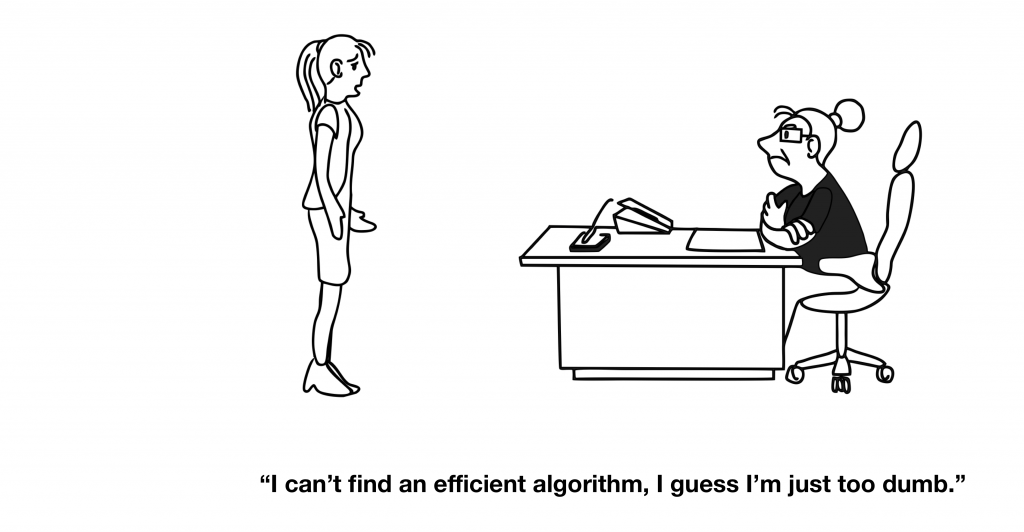
\includegraphics[width=\linewidth]{cartoon.png}
	
	Ideally you'd like to be able to say:
	
	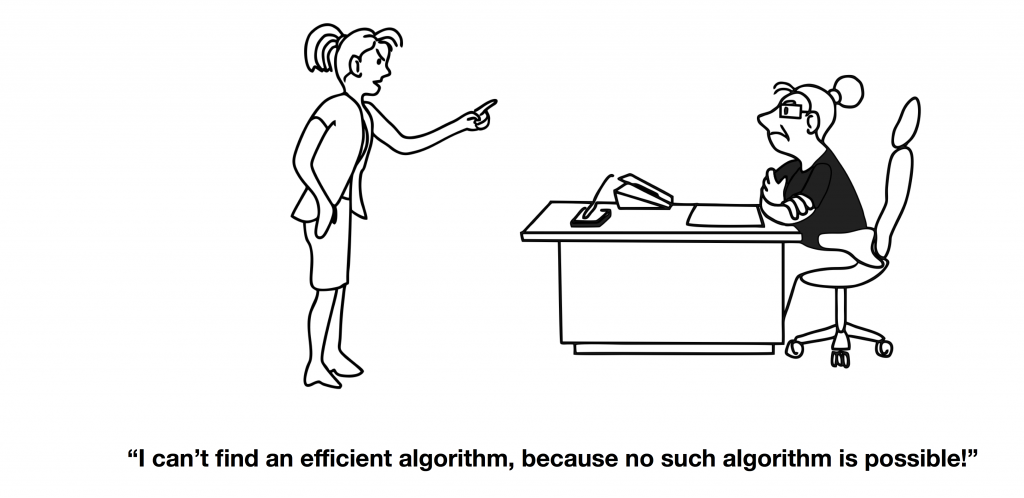
\includegraphics[width=\linewidth]{cartoon2.png}
	
	But in most situations, proving definitively that this is impossible is unlikely.
	\newpage
	
	If you fail to find an efficient solution to a problem, ask yourself: am I struggling to find a solution simply because this is NP-complete? If you can prove it is, you have a great answer for your boss.\\
	
	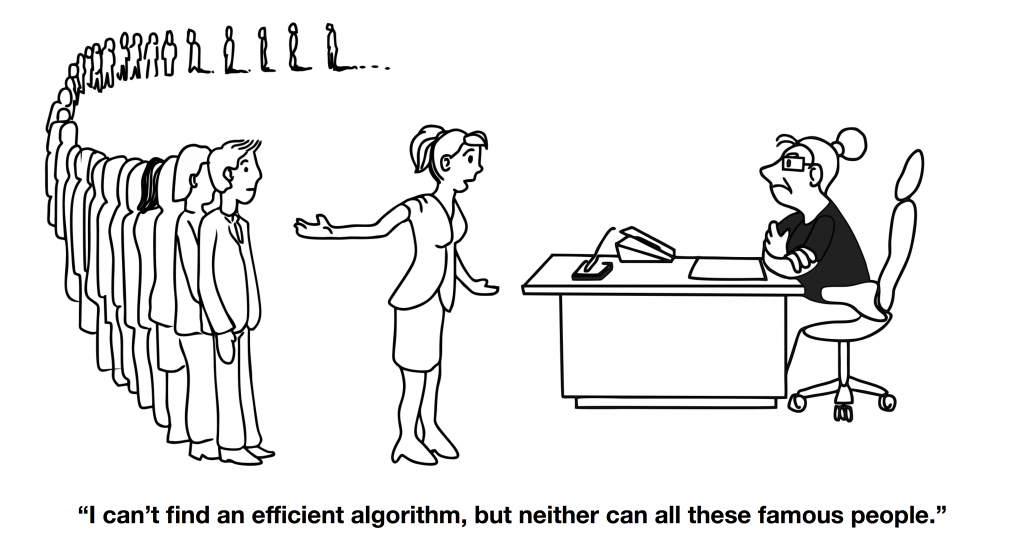
\includegraphics[width=\linewidth]{cartoon3.png}
	
	
	\section{A brief and incomplete history of NP-completeness}
	
	\begin{itemize}
		\item 1971: Stephen Cook proves that every problem in NP can be reduced to a problem called \emph{Boolean Satisfiability} (SAT).\\
		
		In modern terminology: SAT is NP-complete.\\
		
		The same results were developed independently by someone named Leonid Levin, so this is now called the \emph{Cook-Levin} Theorem. \\
		\item 1972: Richard Karp publishes a paper \emph{Reducibility Among Combinatorial Problems}, showing that SAT can be reduced to 21 other problems. \\
		
		
		\item 1979: Garey and Johnson publish the go-to reference on NP-completeness: \emph{Computers and Intractability}.
	\end{itemize}
	
	
	
	
\end{document}